\section{Study on the Influence of Multiple Particle Contacts}\label{sec:contact-study}

In the previous investigations, only two-particle models have been regarded, which is a pretty common approach.
However, two-particle models lack a major influence on the overall sintering response a material shows: the mutual hindering of particles with multiple contacts.
In reality, particle are not able to move freely due to the requirements of a single grain boundary's evolution.
However, particles form complex contacts where the conditions of all involved contacts have influence on each other.

This study shall demonstrate and evaluate this issue on the example of regular sphere packings (circle packing in 2D).

\subsection{Construction of the Study}

\begin{figure}
    \centering
    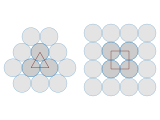
\includegraphics{img/parameter_study/packings}
    \caption{Particle Packings Regarded in this Investigation}
    \label{fig:parameter_study/packings}
\end{figure}

In a regular packing of equal circles each pore in the packing shows equal evolution due to symmetry.
Four different packings, displayed in \cref{fig:parameter_study/packings}, shall be investigated here, which resemble common configurations of sphere packings:
\begin{description}
    \item[Pair] the usual two-particle packing as a reference
    \item[Triangle] the densest possible packing of circles with particles at the corners of an equal sided triangle, resembles a $\left\{ 111 \right\}$ cut through a face-centered cubic cell
    \item[Square] the loosest regular packing with particles at the corners of a square, resembles a $\left\{ 100 \right\}$ cut through a simple cubic cell
    \item[Rhombus] an intermediate packing with particles at the corners of a rhombus of \ang{70}, resembles a $\left\{ 110 \right\}$ cut through a body centered cubic cell
\end{description}
The main difference between these packings is the size and the shape of the pore formed by them.

These packings are expected to show only effects of pore closing, but otherwise behave in a fully symmetric way equivalently to the pair case, as all particles are of equal size, shape and material properties.
In a second step, one of the particles will be given a surface and grain boundary diffusion coefficient \num{1000} times smaller than the other ones to investigate hindering of sintering by the presence of an inert particle.
The term inert shall be used here for a particle with remarkably lower diffusion rate on its surface as well the grain boundary.
This particle is shown with brown stroke in \cref{fig:parameter_study/packings}.
The other ones will be referred as active.

\subsection{Results and Discussion}

\begin{figure}
    \begin{subfigure}{\linewidth}
        \centering
        \includegraphics{sim/packings/shrinkage}
        \caption{Shrinkage}
        \label{fig:packings/shrinkage}
    \end{subfigure}
    \begin{subfigure}{\linewidth}
        \centering
        \includegraphics{sim/packings/neck_size}
        \caption{Average Neck Size}
        \label{fig:packings/neck_size}
    \end{subfigure}%
    \caption{Comparison of Sintering Behavior Obtained for the Investigated Packings}
\end{figure}

\begin{figure}
    \begin{subfigure}{\linewidth}
        \centering
        \includegraphics{sim/packings/cases/pair/evolution}
        \caption{Pure Active}
        \label{fig:packings/pair/evolution}
    \end{subfigure}
    \begin{subfigure}{\linewidth}
        \centering
        \includegraphics{sim/packings/cases/pair_inert/evolution}
        \caption{With Inert Right}
        \label{fig:packings/pair_inert/evolution}
    \end{subfigure}
    \caption{Geometry Evolution of the Pair Cases}
    \label{fig:packings/evolution/pairs}
\end{figure}

\begin{figure}
    \begin{subfigure}{\linewidth}
        \centering
        \includegraphics{sim/packings/cases/triangle/evolution}
        \caption{Pure Active}
        \label{fig:packings/triangle/evolution}
    \end{subfigure}
    \begin{subfigure}{\linewidth}
        \centering
        \includegraphics{sim/packings/cases/triangle_inert/evolution}
        \caption{With Inert Upper}
        \label{fig:packings/triangle_inert/evolution}
    \end{subfigure}
    \caption{Geometry Evolutions of the Triangle Cases}
    \label{fig:packings/evolution/triangles}
\end{figure}

\begin{figure}
    \begin{subfigure}{\linewidth}
        \centering
        \includegraphics{sim/packings/cases/square/evolution}
        \caption{Pure Active}
        \label{fig:packings/square/evolution}
    \end{subfigure}
    \begin{subfigure}{\linewidth}
        \centering
        \includegraphics{sim/packings/cases/square_inert/evolution}
        \caption{With Inert Upper-Right}
        \label{fig:packings/square_inert/evolution}
    \end{subfigure}
    \caption{Geometry Evolutions of the Square Cases}
    \label{fig:packings/evolution/squares}
\end{figure}

\begin{figure}
    \begin{subfigure}{\linewidth}
        \centering
        \includegraphics{sim/packings/cases/rhombus/evolution}
        \caption{Pure Active}
        \label{fig:packings/rhombus/evolution}
    \end{subfigure}
    \begin{subfigure}{\linewidth}
        \centering
        \includegraphics{sim/packings/cases/rhombus_inert/evolution}
        \caption{With Inert Upper}
        \label{fig:packings/rhombus_inert/evolution}
    \end{subfigure}
    \caption{Geometry Evolutions of the Square Cases}
    \label{fig:packings/evolution/rhombii}
\end{figure}

\Cref{fig:packings/shrinkage} shows the shrinkage for the distinct packings obtained from the simulations.
The shrinkage is calculated in all cases using the polygon approach as discussed in \cref{sec:packings}, except for the pair for which the polygon approach is not applicable and so the distance approach is used.
Note, that the distinct cases all show the equal behavior in early stages and the two approaches to shrinkage calculation are equivalent.
At some point, specific to the respective case, the curve deviates rapidly to higher shrinkages from the reference two-particle model.
This point is related to the pore closing and the change of its shape characteristic from concave to convex, as is discussed in \textcite{Tikare2003}.
Therefore, the deviation occurs earlier for the more dense packed cases, in order: triangle, rhombus, square.
\textcite{Jing2003} reported \gls{PFM} simulations of a single pore which first show the deviation to the upper side, also observed here, and then the transition into steady state when the pore was fully closed.
The effect there is likely not that pronounced as here, since the \gls{PFM} approach blurs the pore due to the diffuse interface which acts like a regularization when the pore size is similar to the numerical interface width.

At the point where the pore was completely closed, the simulations were cancelled, since the current model does not support triple points yet.
As the model is only aimed at initial and intermediate sintering stages, this problem can be neglected.
Complete closure was determined at the point, were the last surface node between two neck nodes was removed by the neck remeshing procedure.
Note that equal colors represent equal times in all cases.
The shrinkage response shows a drastic increase in slope prior to pore closing, as the curvature of the pore increases while its size decreases.
This enhances the driving force.

\Cref{fig:packings/neck_size} shows the neck sizes for the distinct packings obtained from the simulations.
The curve drawn represents the average of all necks for the multiple-particle cases.
The general trends are the same as for shrinkage.
The beginning of pore closing is first noticed by a deviation to the lower from the straight line.
As the pore closes further, the neck growth rate increases drastically so that the neck size curve crosses the straight again.

The cases with an inert particle show a remarkably lower shrinkage and neck size, since the contribution of volume removed from the grain boundary of the inert particle is missing.
This is in accordance with experimental observations \cite{German2014}.
The numerical behavior of all cases with an inert particle is remarkably worse than of the pure active cases, as is apparent from the kinks in the result curves.
The detailed logs of the simulation suggest the reason to the more erratic neck remeshing on the inert particle.
The pore closing is delayed as the pore is kept open by the inert particle's surface.
The three multiple-particle packings with an inert behave similarly, show equal behavior in early stages and pore closing occurs in the same order as for the pure active cases.
The pair with an inert shows a distinct behavior to the other inert cases.
Its shrinkage is the lowest.
A correlation with the count of active particles present seems unlikely, since the two-particle case is the only one behaving differently.
\textcite{German2014} reported possible crack formation in the active-active and the active-inert interfaces due to tension stresses occurring, since the inert particle inhibits free and uniform particle movement.
This did not occur in the current investigations, likely because the inert particle was not fully surrounded by active particles.
Nevertheless, the simulation would currently cancel if a neck shrinks and approaches zero width, as contact release is not implemented.

Looking at the geometry evolutions in \crefrange{fig:packings/evolution/triangles}{fig:packings/evolution/rhombii}, the convexity respectively concavity of the pore can clearly be observed.
The pore surface to the inert particle stays concave during the whole process.
As previously observed in \cref{subsec:parameter-study-asymmetric-surface-diffusion-ratio}, the grain boundaries between inert and active particles are curved, since the active particle creeps around the inert one.
On the inert particle an undercut evolves near the neck.
The remaining pore volume at the state of simulation cancellation is significantly higher than in the pure active cases.
